\chapter{\label{method}Method}

The question to be researched is whether an adaptive bucket-table can be made to do ranking more efficient than a static table with offline updates.

\section{Problem description revisited}

The Companys current ranking algorithm is an implementation of the algorithm \emph{Bucket with Global Query} (See \labelcref{bucket}). The highscores are stored in Google App Engines Datastore as entities with properties \emph{username} and a \emph{highscore}. When a player gets a new highscore it replaces the old highscore.

Since score in this case is measured in milliseconds and lower timings are better a better score is a lower number\footnote{While this really should not matter at all, be aware that this fact is a good foundation for getting mindfucked very hard}.

A background job  periodically iterates through all the highscores making the bucket-table that contains ranks and scores needed to make the estimates. The entities are indexed on highscore-property which is essential to make the process of iterating through the whole set doable.

\todo{Following examples on how the algorithm operates should be moved to previous chapter}

An exerpt from the bucket-table may look like table \ref{table:ranking-table}. For example, to estimate rank for score $2\;050$ which falls in bucket 6, start by calculating what the score range in bucket 6 is, in this case $2\;204 - 1\;961 = 243$. $2\;050$ is $89$ scorepoints in the bucket and hence the rank is calculated as $83 + 23 \times \frac{89}{243} \approx 91$. See figure \ref{fig:interpolation} for a visual representation of the example.

\begin{table}[h]
  \begin{center}
  \begin{tabular}{ c c c c }
    Bucket no & Start score & Start rank & Size \\
    5 & 1 515 & 83 & 22 \\ 
    6 & 1 961 & 105 & 23 \\ 
    7 & 2 204 & 128 & 23 \\ 
    8 & 2 574 & 151 & 24 \\  
    9 & 2 852 & 175 & 25 \\ 
  \end{tabular} 
  \caption{Excerpt from bucket-table}
  \label{table:ranking-table}
  \end{center}
\end{table}

\begin{figure}[h!]
  \centering
  \caption{Linear interpolation of rank for score 2050}
  \label{fig:interpolation}
  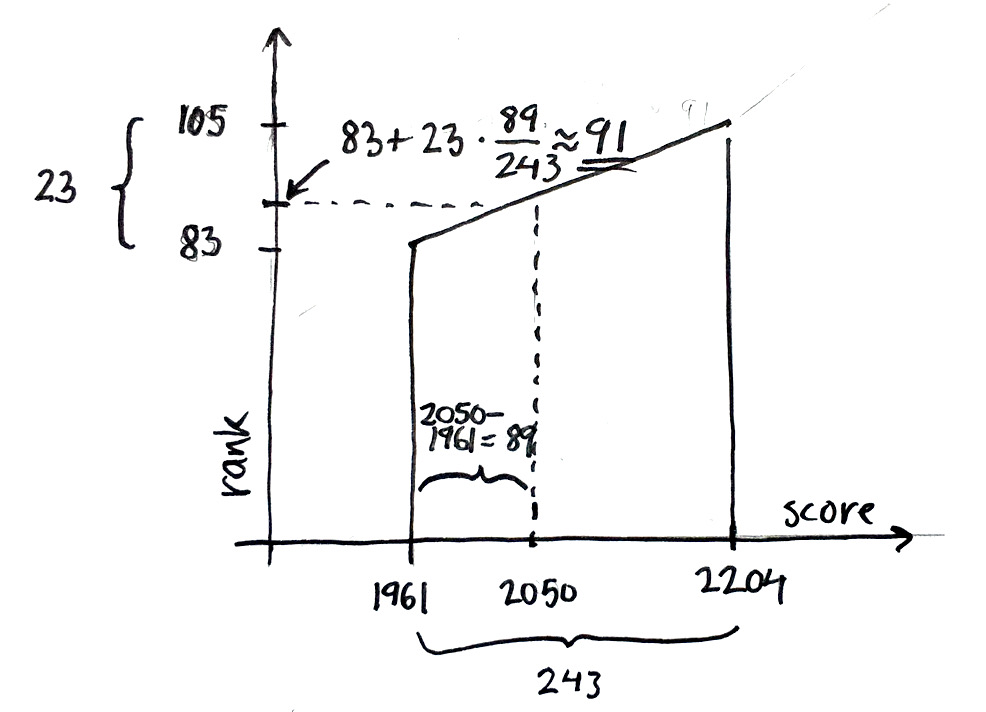
\includegraphics[width=8cm]{img/interpolation.jpg}
\end{figure}

If an update of a highscore from a lower one score to a higher occurs but the new score is within the the same bucket as the previous one, the subsequent estimate will be the same for any score since the bucket-table is unchanged. Because the underlying distribution is changed the error may be different but not necessarily worse.

\todo{This is not 100 \% correct}

On the other hand, if a highscore estimate goes from a lower rank bucket to a higher one, a subsequent scan of the highscores would result in a table where the new bucket will grow by one and, start-rank of buckets after the new to and including the former one will increase by one and the bucket for the previous estimate would shrink by one. Se figure \ref{fig:change-buckets}.

\todo{Illustration}

% \begin{figure}[h]
%  \centering
%  \caption{A new highscore breaking the bucket-table}
%  \label{fig:change-buckets}
%  
\includegraphics[width=8cm]{img/change-buckets.png}
%\end{figure}

Future high scores will add to the bucket-tables deviation from a theorethical \emph{true} bucket-table and as a consequence rank estimates will show a growing error with respect to the true rank until the bucket-table is recreated (Figure \ref{fig:errortime}).

\begin{figure}[h]
  \centering
  \caption{Error over time}
  \label{fig:errortime}
  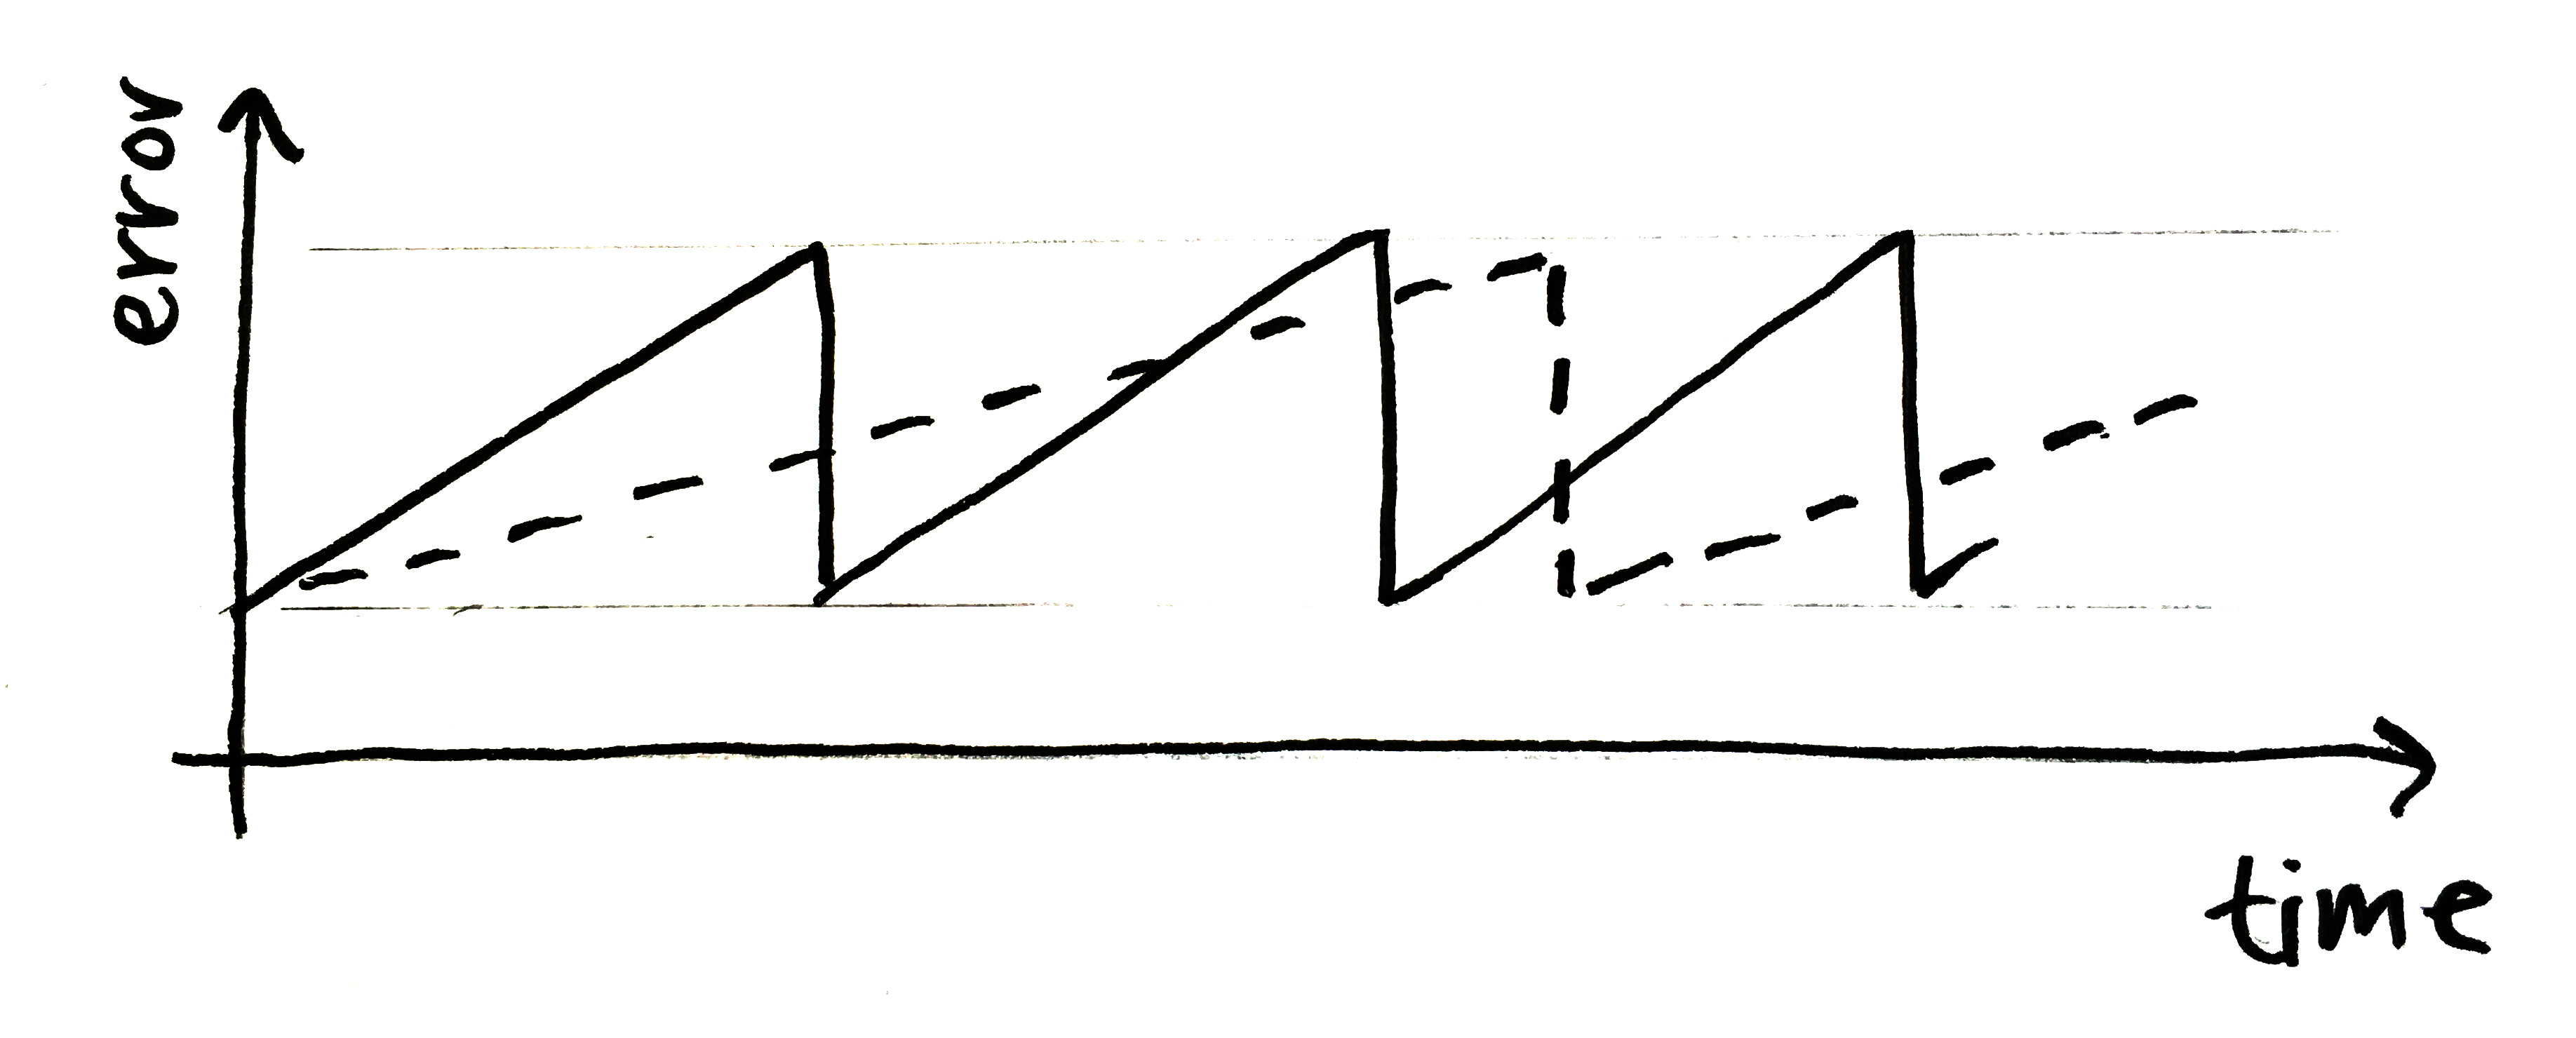
\includegraphics[width=8cm]{img/hypothesis2.jpg}
\end{figure}

\section{Hypothesis} 

The current implementation starts a background job that builds the bucket-table every ten minutes. When the scan is complete a reference is set to the new table and the old one is discarded. The accumulated error is at its maximum right before the switch and will in the forthcoming reasonings serve as an upper limit for what would be an acceptable performance.

The total cost for providing the ranking service with the current implementation and the implementation to be assessed is $n \times costforestimate + \frac{ costfortablecreation}{n}$.

\todo{Better formula}

\todo{Rewrite hypothesis}

The hypothesis is as follows:

\blockquote{Running the ranking service with the new implementation will be more efficient than the current implementation at the same level of error.}

\begin{figure}[h]
  \centering
  \caption{Cost vs time. Dotted line is the outcome when hypothesis the hypothesis is true.}
  \label{fig:cost}
  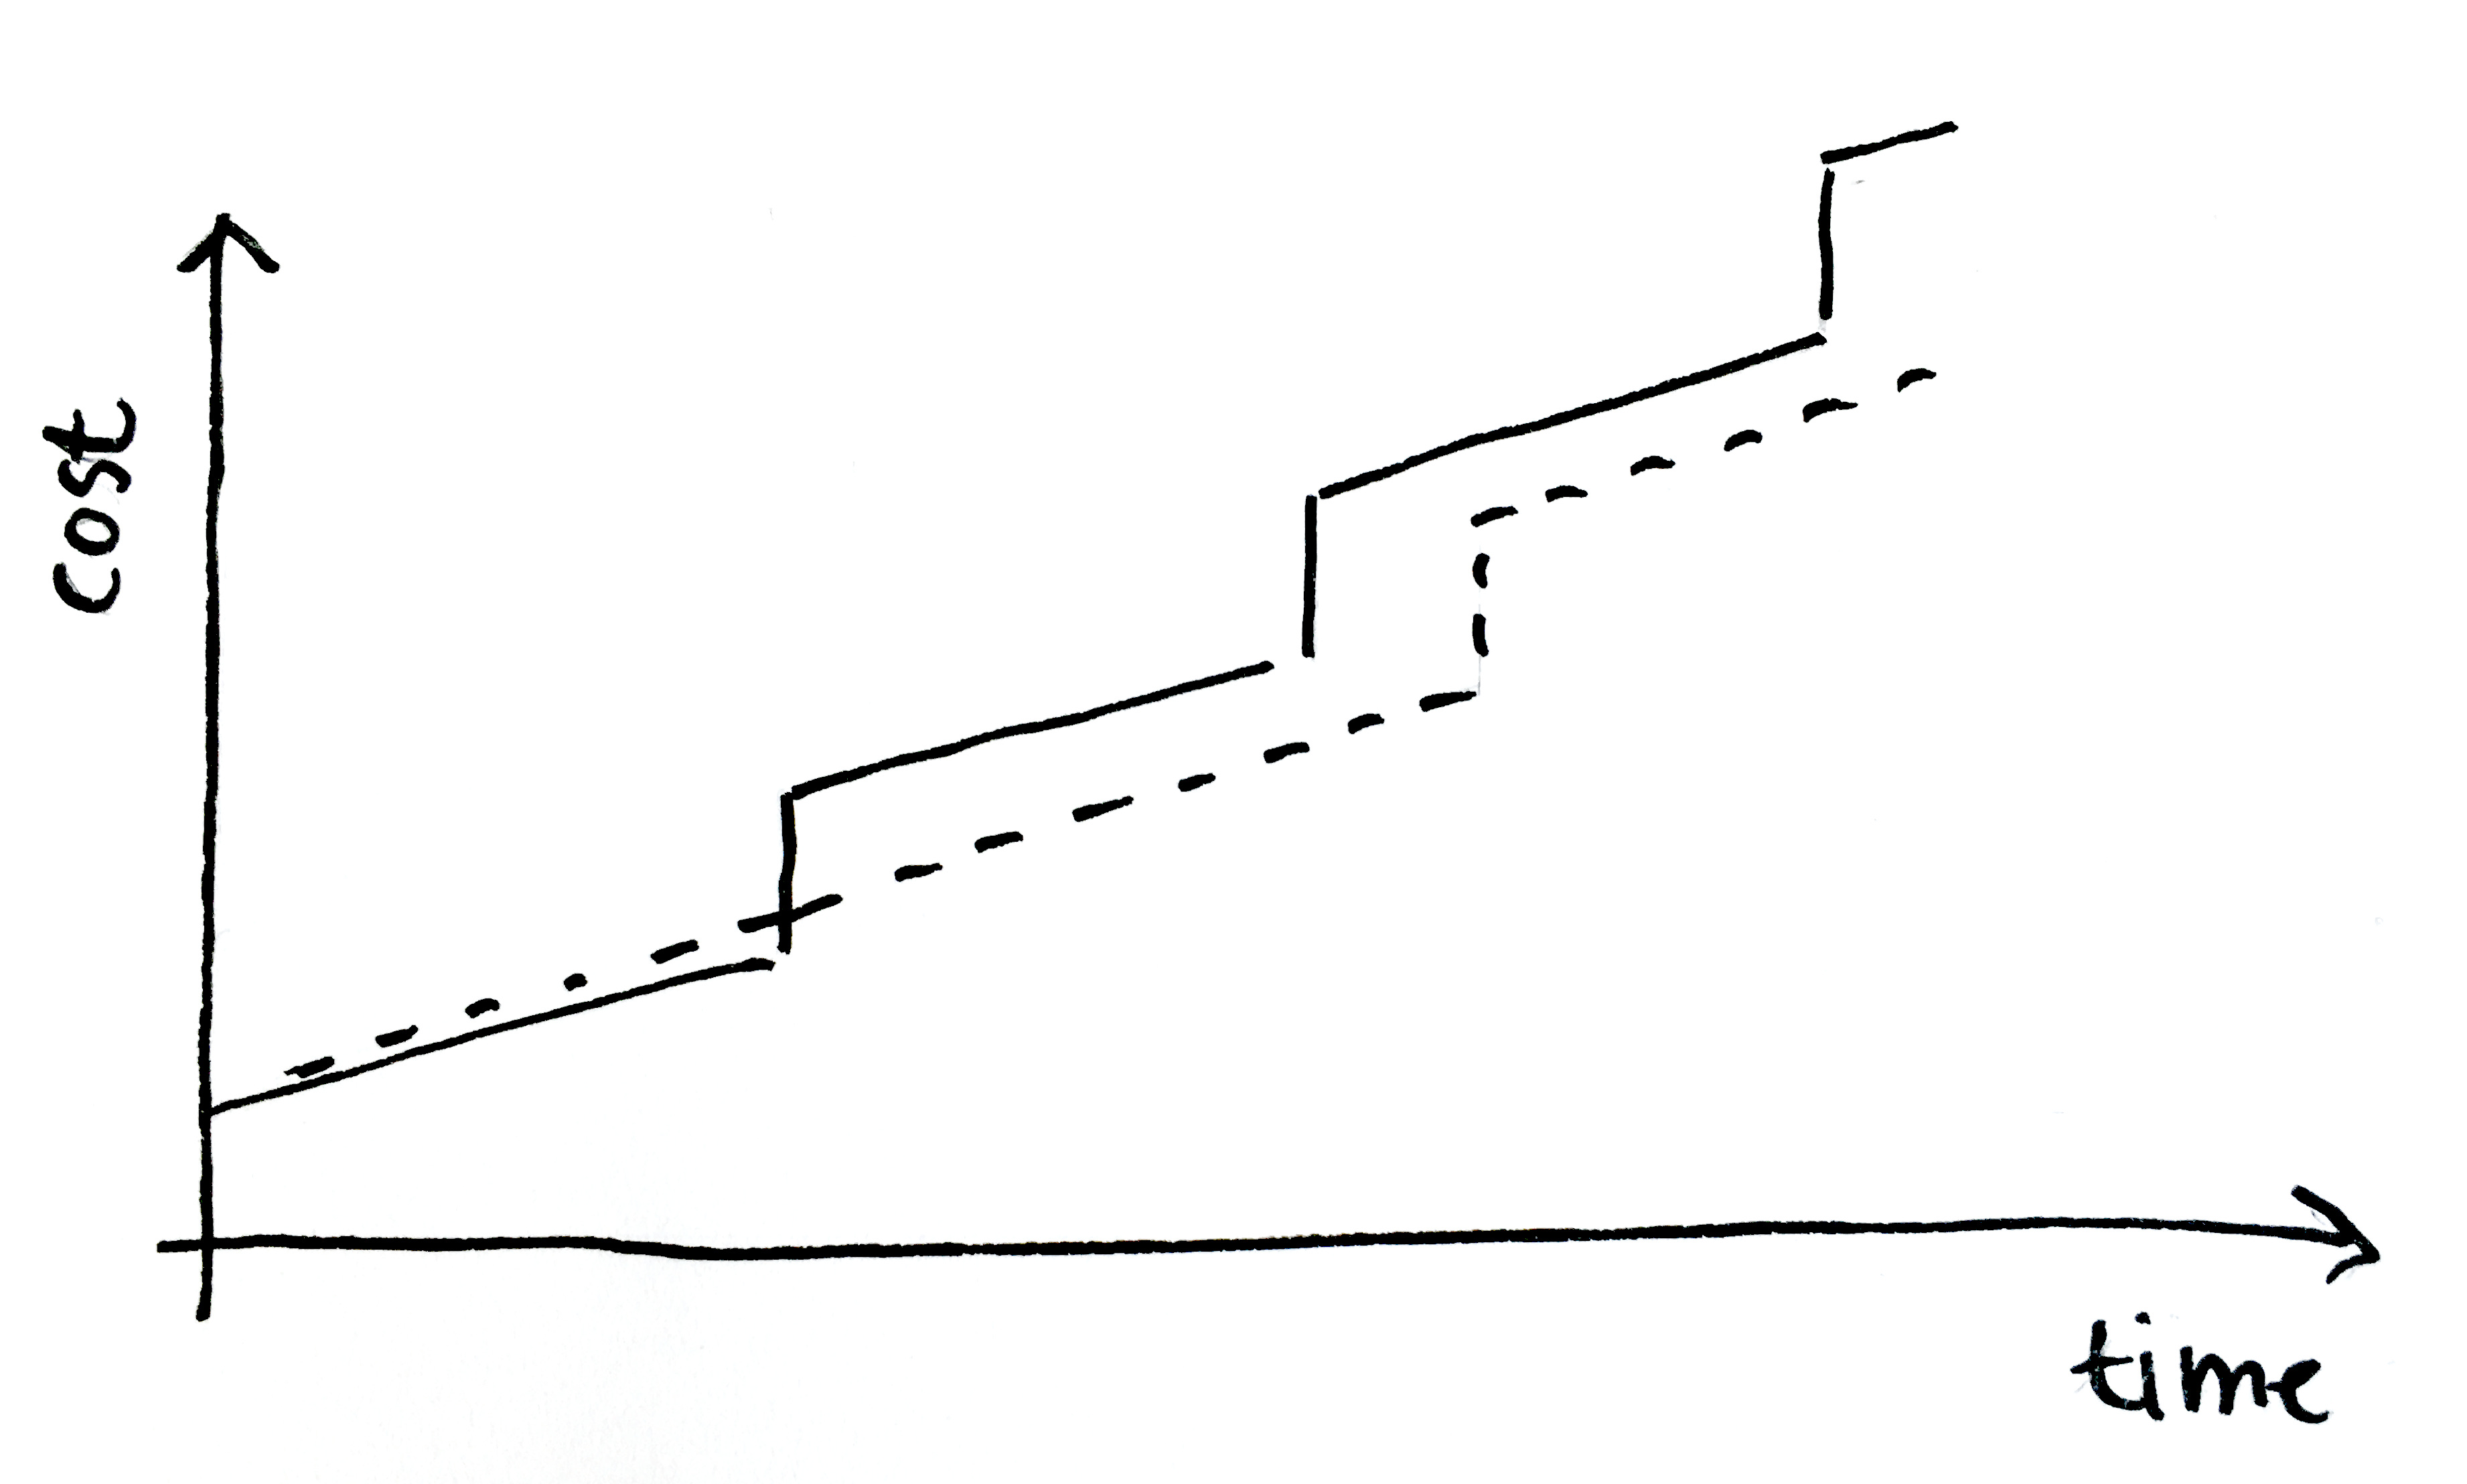
\includegraphics[width=8cm]{img/hypothesis.jpg}
\end{figure} 


\section{Data}

In this experiment only synthetic data will be used. The choice is both practical and a methodologically motivated. First, the production system cannot be altered in such a way that real world data could be tapped within this experiments ,timeframe. Also, real world data in this system differs from one time period to another both in terms of the highscore distribution and throughput -- and of course, data from one application differs from data from other applications. Using synthetic data make the results more general.

\todo{Something about the data used in test}

\todo{Same random seed is always used}

\section{What and how to measure}

To be able to test the hypothesis relative error and execution time will be logged per ranking request.

For the \emph{true} value for calculating the relative error, an exact rank is calculated for that instant. While using other values as true values, such as values created with a fresh bucket-table every time, the exact value seemed to be the most predictable option.

The execution time is measured by calls to \texttt{System.currentTimeInMillis()} in the servlet receiving the ranking request.

\section{The experiment}

The experiment is implemented in a client-server-model where the client simulate playing a game and sends highscores to the server. The server responds with an estimated rank and the execution time for processing the request. The client is a regular Java program with no bells and whistles and the server consists of a number of servlets designed to run on Google App Engine. 

The test environment is set up by resetting or generating the 100 000 highscore entries with random highscores. Lower number means higher score. The highscores have a Gaussian distribution which is somewhat similar to the distribution of real-world highscores\footnote{The real world highscores are similarly distributed to each other and somewhat similar to a Gaussian distribution. However, no effort has ben made to do a statistical analysis of them.}

\todo{Be more precise about the distribution}

When the client has finnished ``playing'' a round it always get a new highscore. The new highscore is better than the old one by a number drawn from a uniform pseudorandom distribution $1-1000$.

To be able to measure the relative error of the estimates the client starts by asking for a list of all highscores. When the client sends a new highscore to the server it also updates its local highscore list. When the server responds with the rank estimate for the new score, that estimate is compared with the real rank and ultimately used for calculating the relative error.

The type of ranking algorithm to use is set before starting the test.

\subsection{Technical details}

The Companys original implementation of the ranking algorithm is written in Java and runs on Google App Engine and. So is this experiment. This is an overly complicated infrastructure to perform the experiments in as the same results could have been gained with a simple command-line interface application not communicating over HTTP at all. The choice is motivated by the initial ambitions that were a lot higher than the actual outcome.

\subsubsection{Libraries}

A few libraries are used; \emph{Objectify} which provides means for persisting Java objects to the App Engines Datastore
and \emph{Jackson} for parsing and generating JSON-data. Naturally, the App Engine SDK is also used.

\todo{Make list and references}

\section{Limitations}

\todo{The real world data set grows over time. Will be ignored, only focus on case when the set of highscores are reasonably large.}

\todo{Only tested on development server}
